\documentclass[letter,11pt]{article}

\usepackage[spanish,es-nodecimaldot]{babel}
\usepackage[utf8]{inputenc}

\usepackage{lmodern}
\usepackage[T1]{fontenc}
\usepackage{textcomp}

\usepackage{framed}
\usepackage[svgnames]{xcolor}
\colorlet{shadecolor}{Gainsboro!50}

\usepackage{enumitem}
\usepackage{graphicx}
\usepackage{pstricks}

\usepackage{anysize}
\marginsize{3cm}{2cm}{2cm}{3cm}

\usepackage{siunitx}
\usepackage{amsmath}
\usepackage{array}
\usepackage{alltt}

\usepackage{fancyhdr}
\usepackage{lastpage}
\pagestyle{fancy}
\fancyhf{}
\fancyhead[LE,RO]{Física Básica III}
\fancyfoot[CO,CE]{\thepage\ de \pageref{LastPage}}

\special{papersize=215.9mm,279.4mm}

\usepackage[
    pdfauthor={Carlos Eduardo Caballero Burgoa},%
    pdftitle={Física Básica III},%
    pdfsubject={Tarea},%
    colorlinks,%
    citecolor=black,%
    filecolor=black,%
    linkcolor=black,%
    urlcolor=black,
    breaklinks]{hyperref}
\usepackage{breakurl}

\newcommand{\blankpage}{
\newpage
\thispagestyle{empty}
\mbox{}
\newpage
}

\renewcommand{\arraystretch}{1.2}

\begin{document}

\begin{center}
    {\Large \bf{\underline{Tarea}}}
\end{center}

Calcular la fuerza eléctrica ($F_E$) en $q$, dado que: $q = -2[\mu C]$,
$q_1 = +1[\mu C]$, $q_2 = +2[\mu C]$, $q_3 = -1[\mu C]$, $q_4 = +3[\mu C]$, 
$a = 5[cm]$, $b = 3[cm]$.

\begin{figure}[!h]
\centering
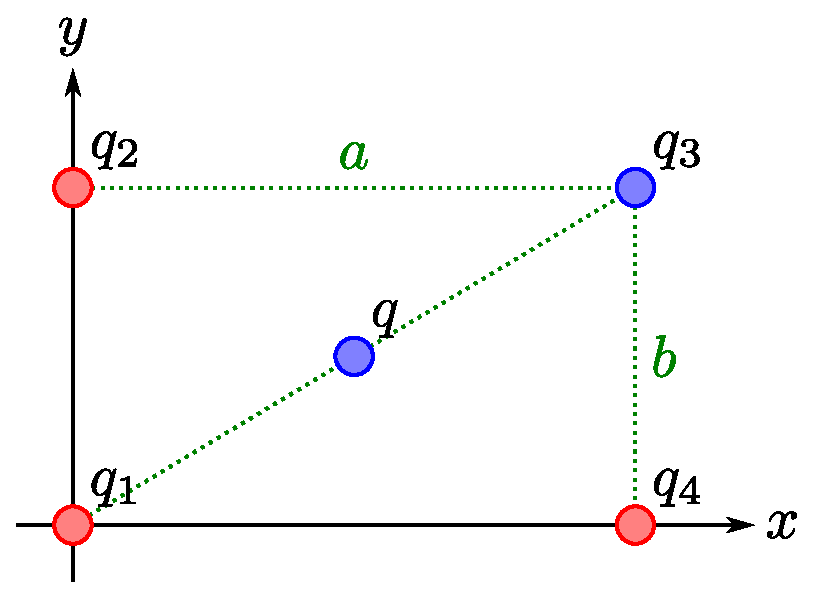
\includegraphics[scale=0.45]{resources/f1.eps}
\end{figure}

\vspace{0.5cm}
\textbf{\underline{Solución}:} \\

Los vectores de posición de las cargas son:

\begin{equation*}
    \vec{r} = 0.025 \hat{u}_x + 0.015 \hat{u}_y [m]
\end{equation*}
\begin{equation*}
    \vec{r}_1 = 0 \hat{u}_x + 0 \hat{u}_y [m]
\end{equation*}
\begin{equation*}
    \vec{r}_2 = 0 \hat{u}_x + 0.03 \hat{u}_y [m]
\end{equation*}
\begin{equation*}
    \vec{r}_3 = 0.05 \hat{u}_x + 0.03 \hat{u}_y [m]
\end{equation*}
\begin{equation*}
    \vec{r}_4 = 0.05 \hat{u}_x + 0 \hat{u}_y [m]
\end{equation*}

\vspace{0.5cm}
Por tanto $\vec{F}_E$ es:

\begin{equation*}
    \vec{F}_E = \sum_{i=1}^4 \frac{1}{4 \pi \epsilon_0} q q_i \frac{\vec{r} - \vec{r}_i}{|\vec{r} - \vec{r}_i|^3}
              = \frac{q}{4 \pi \epsilon_0} \sum_{i_1}^4 q_i \frac{\vec{r} - \vec{r}_i}{|\vec{r} - \vec{r}_i|^3}
\end{equation*}
\begin{equation*}
    \vec{F}_E = \frac{q}{4 \pi \epsilon_0} \left(
        q_1 \frac{\vec{r} - \vec{r}_1}{|\vec{r} - \vec{r}_1|^3} +
        q_2 \frac{\vec{r} - \vec{r}_2}{|\vec{r} - \vec{r}_2|^3} +
        q_3 \frac{\vec{r} - \vec{r}_3}{|\vec{r} - \vec{r}_3|^3} +
        q_4 \frac{\vec{r} - \vec{r}_4}{|\vec{r} - \vec{r}_4|^3} \right)
\end{equation*}

\vspace{0.5cm}
Calculando el valor de las diferencias, obtenemos:

\begin{equation*}
    \vec{r} - \vec{r}_1 = 0.025 \hat{u}_x + 0.015 \hat{u}_y - 0 \hat{u}_x - 0 \hat{u}_y = 0.025 \hat{u}_x + 0.015 \hat{u}_y
\end{equation*}
\begin{equation*}
    \vec{r} - \vec{r}_2 = 0.025 \hat{u}_x + 0.015 \hat{u}_y - 0 \hat{u}_x - 0.03 \hat{u}_y = 0.025 \hat{u}_x - 0.015 \hat{u}_y
\end{equation*}
\begin{equation*}
    \vec{r} - \vec{r}_3 = 0.025 \hat{u}_x + 0.015 \hat{u}_y - 0.05 \hat{u}_x - 0.03 \hat{u}_y = - 0.025 \hat{u}_x - 0.015 \hat{u}_y
\end{equation*}
\begin{equation*}
    \vec{r} - \vec{r}_4 = 0.025 \hat{u}_x + 0.015 \hat{u}_y - 0 \hat{u}_x - 0.03 \hat{u}_y = - 0.025 \hat{u}_x + 0.015 \hat{u}_y
\end{equation*}
\begin{equation*}
    |\vec{r} - \vec{r}_1| = |\vec{r} - \vec{r}_2| = |\vec{r} - \vec{r}_3| = |\vec{r} - \vec{r}_4| = 0.029155
\end{equation*}
\begin{equation*}
    |\vec{r} - \vec{r}_i|^3 = \num{2.4782e-5}
\end{equation*}

\vspace{0.5cm}
Resultando:

\begin{equation*}
\begin{split}
    \vec{F}_E =
        \left[ \frac{\num{-2e-6}}{4\pi(\num{8.8542e-12})} \right]
        \Biggl[ (\num{1e-6})\frac{(0.025 \hat{u}_x + 0.015 \hat{u}_y)}{\num{2.4782e-5}}+
    \\
        (\num{2e-6})\frac{(0.025 \hat{u}_x - 0.015 \hat{u}_y)}{\num{2.4782e-5}}+
    \\
        (\num{-1e-6})\frac{(-0.025 \hat{u}_x - 0.015 \hat{u}_y)}{\num{2.4782e-5}}+
    \\
        (\num{3e-6})\frac{(-0.025 \hat{u}_x + 0.015 \hat{u}_y)}{\num{2.4782e-5}} \Biggr]
\end{split}
\end{equation*}
\begin{equation*}
    \vec{F}_E = (-18.134 \hat{u}_x -32.640 \hat{u}_y) [N]
\end{equation*}

\end{document}

